%-------------------------------------------------------
\section{Available Data}
%-------------------------------------------------------
\begin{frame}{Raw Data}{What is the nature of the starting material?}
%-------------------------------------------------------

\begin{itemize}

    \item<1->\textbf{Data about \alert{students}}: academic career results of each student during a certain time span \\
        \noindent\begin{centering}
            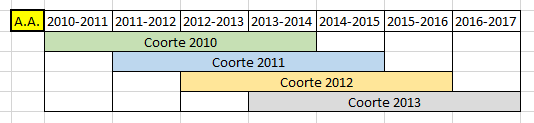
\includegraphics[scale=0.50]{../raw/stud_comp.png}
        \end{centering}

    \item<2->\textbf{Data about \alert{courses}}: teachings evaluations questionary compiled by the students, in an \emph{aggregate} form for each \texttt{<Academical Year, Teaching Course>}.

\end{itemize}

\end{frame}

%-------------------------------------------------------
\section{Data Understanding}
%-------------------------------------------------------
\subsection{Students Data}
%-------------------------------------------------------
\begin{frame}{Data Understanding}{Visualization techniques on students general results}

    \begin{centering}
        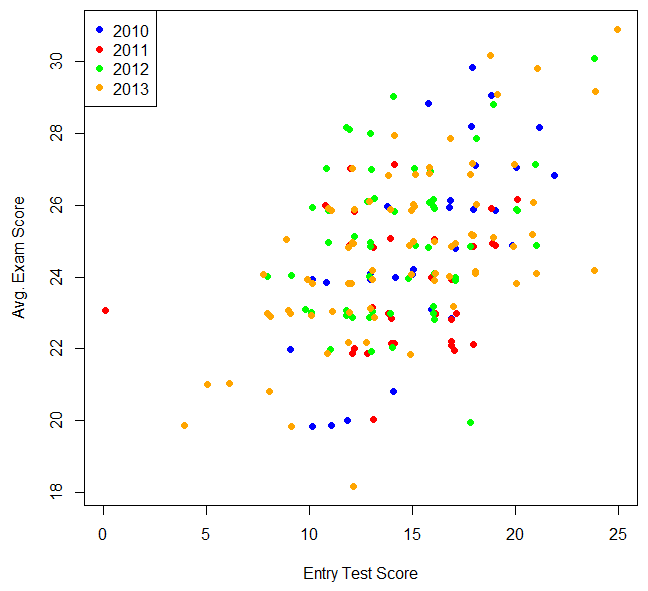
\includegraphics[scale=0.46]{../thesis/img/scatter_plot_2.png}
    \end{centering}

\end{frame}

\begin{frame}{Data Understanding}{Visualization techniques on students first year exams results}

    \begin{centering}
        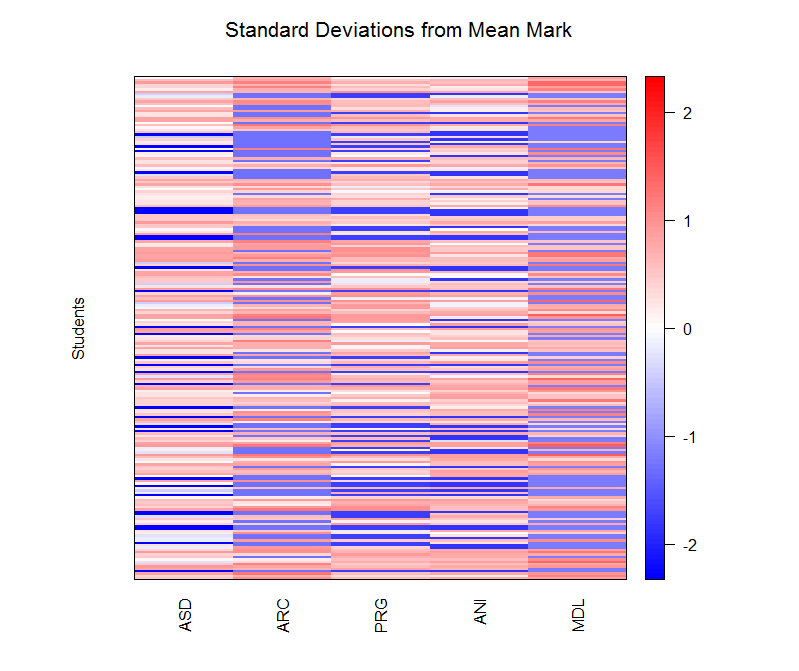
\includegraphics[scale=0.47]{../thesis/img/std_dev_matrix_1.png}
    \end{centering}

\end{frame}

\begin{frame}{Data Understanding}{Visualization techniques on students I.T. exams results}

    \begin{centering}
        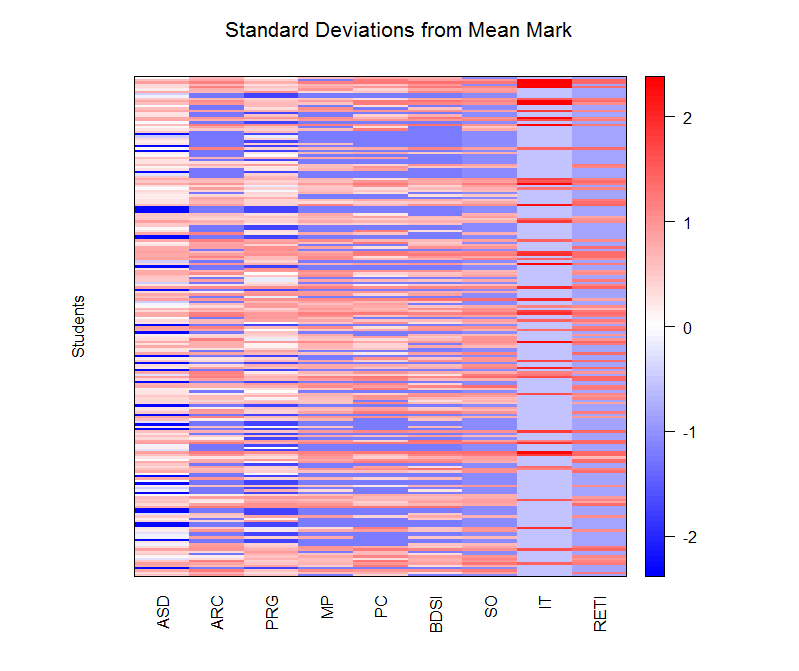
\includegraphics[scale=0.48]{../thesis/img/std_dev_matrix_2.png}
    \end{centering}

\end{frame}

\begin{frame}{Data Understanding}{Visualization techniques on students math exams results}

    \begin{centering}
        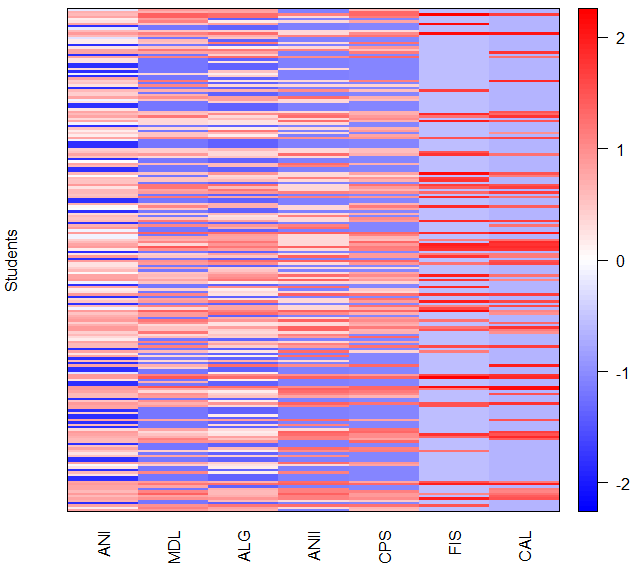
\includegraphics[scale=0.48]{../thesis/img/std_dev_matrix_3.png}
    \end{centering}

\end{frame}